\chapter{Homology}
\label{chapter5}

In this chapter we will shift our attention back to algebraic topology and more specifically the field of Homology. We will use Homology to analyse the connectivity, number of the holes and voids in a simplical complex. We are putting all this work in Homology because it is a prerequisite to one of the leading tools in topological data analysis - Persistent Homology. In the next chapter we will analyse some of the similarities between persistent homology computations and contour tree computations.

\section{Homology}


% @TODO Fix introduction

The guiding principle behind the Euler Characteristic was to decompose a space into cells, count them and perform cancellations based on the parity of the dimension of the cells. This approach yields valuable information about a topological space, but we can hope to gain more by generalising it. We shall accomplish this by leveraging the mathematical machinery of Homology. Homology is a tool that was first developed to measure the topological complexity of manifolds \cite{persistence-original}. For example with homology we can recognize that there is a hole in the torus and a volume enclosed in the sphere. The theory of Homology comes in two flavours - \textbf{simplical} and \textbf{singular}. Simplicial homology is geared towards analysing simplical complexes and singular homology is the appropriate generalisation for arbitrary topological spaces. In this dissertation we restrict attention on singular homology because we are primarily interested in the computational aspect of homology.

%We will however on occasion refer to singular homology when we desire to leverage a more general result from the relevant theory. More information on singular homology can be found in the following sources \cite{algebraic-topology, elementary-applied-topology}


Homology is built around the interplay between two key concepts of \textbf{cycles} and \textbf{boundaries}. Let us consider the simplical complex depicted on Figure \ref{fig:hom-sc} as an example. It consists of four vertices $\{a, b, c, d\}$, five edges $\{ab, bc, ca, db, cb\}$ and one face $\{abc\}$. Let us first explain what a boundary is. The boundary of a simplex consists of its codimension-1 faces. For example the boundary of the 1-dim simplex $ab$ consists of the 0-dim simplices $a \text{ and } b$. The boundary of the 2-dim simplex $abc$ consists of the 1-dim simplices $ab, ac \text{ and } cb$. A cycle on the other hand consists of the simplices that form the boundary of a simplex that is of one dimension higher (regardless of whether that one dimension simplex is in the complex). In our example we can observe that the edges $ab, bc, ca$ and $bd, dc, cb$ form a 1-dim cycle because they are the boundary of the-dimensional simlices $abc$ and $bdc$. The first simplex $abc$ is in the complex while $bdc$ is not. The definition of one dimensional cycles is in line with the graph theoretic definition. The first and last vertex of the paths formed by those edges are the same. A more geometric way to put it is that the edges enclose an 2-dim area of space. To expand this definition to higher dimensional cycles picture the faces of the tetrahedron. They would form a 2-cycle as they completely enclose a 3-dim volume. In general an n-cycle consists of simplices that are the boundary of a n+1-dim simplex

\begin{figure}[h]%
    \centering
    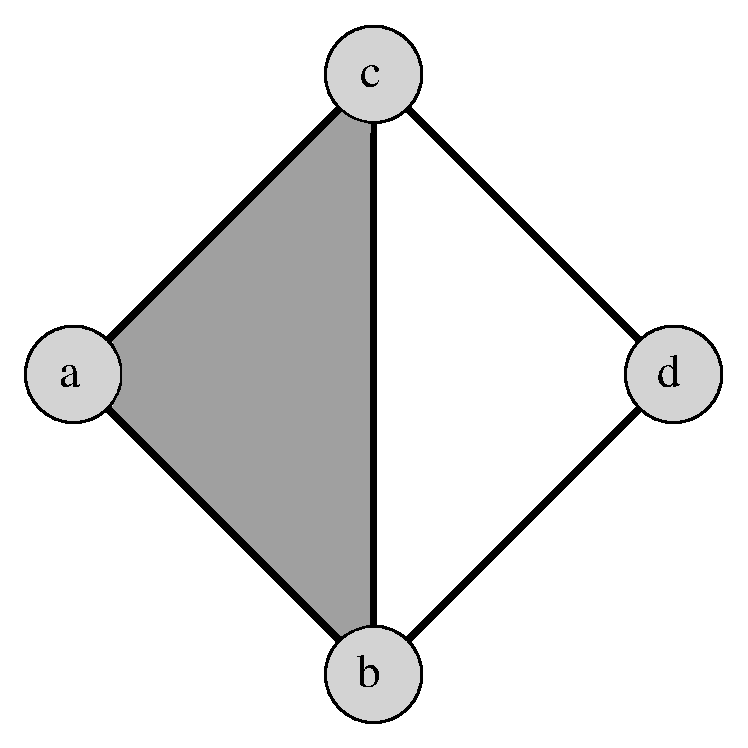
\includegraphics[scale=0.4]{./images/chapter1/homology-sc.eps}%
    \caption{An Example Simplical Complex}%
    \label{fig:hom-sc}%
\end{figure}

The interplay between between cycles and boundaries is in asking the question - which cycles in the complex are \textbf{not} the boundary of a higher dimensional simplex. Such cycles are important because they introduce a void in the space. Cycles which are the boundary of a higher dimensional simplex can be disregarded because the void they introduces is filled by that higher dimensional simplex. Coming back to our example the cycle $ab, bc, ac$ is the boundary of $abc$, but the cycle $db, cd, bc$ it not the boundary of another simplex in the simplical complex. The cycle $db, cd, bc$ represents a 2-dim hole in the simplical complex. Finally note that the cycle $ab, bd, dc, ac$ is in a sense equivalent to the cycle $db, cd, bc$ because both describe the same 2-dim hole in the complex - namerly the missing 2-dim simplex $bdc$.

%This is important because these cycles cannot be contracted to a point. The lack of higher dimensional simplex the enclose means there is a void of some dimension in our simplex.

Notice also that the paths formed by the edges $bc, ca, ab$ and $ac, ab, bc$ represent the same cycle. The only difference is which vertex is the starting and ending point. We would like to disregard the choice of starting point and order of edges completely because for example the paths $bc, ac, ab$ and $ac, ab, bc$  represent the same structure in the simplical complex. Enter additive algebraic notation. In this notation the same cycle would be written as $ab + bc + ca$.

Additive notation implies associativity but it does not have to sole purpose of illustrating the point of disregarding edge order. Its more important aspect is that it allows us to treat sums of edges as linear combinations in an abstract vector space. To begin with, we will operate with vector spaces over the field of coefficients $\mathbb{Z}_2 = \{0, 1\}$ together with the standard operations of addition and multiplication modulo two. We will use abstract vector spaces over the field of coefficients $\mathbb{Z}_2$ as the building blocks of our study of Homology.

Let $X$ be a simplicial complex. An n-chain of $X$ is a formal sum of n-simplices of $X$ \cite{comp-topo}. The notation we will use for an n-chain is $\sum{a_i \sigma_i}$ where $a_i \in \mathbb{Z}_2$ and $\sigma_i$ is an n-simplex of $X$. We can add two n-chains component wise much like we would add polynomials. For example $(ab + bc) + (ab + cd + db) = 2ab + bc + cd + db = bc + cd + bd$ because $2 = 0$ in $\mathbb{Z}_2$.

Based on the n-chains of $X$ we can define the \em chain complex \em of $X$. It is made up of the following vector spaces and linear maps between them:

\begin{itemize}

    \item The \textbf{group of n-chains} $C_n(X)$ of $X$. These are the vector spaces where the vectors are all possible n-chains of $X$ and the coeficients are $\mathbb{Z}_2$.

    \item The \textbf{boundary maps} $\partial_n$ between the groups of n-chains of $X$. These are linear maps between consecutive groups of n-chains $\partial_n : C_n(X) \to C_{n-1}(X)$.

\end{itemize}

What we have defined as the chain complex of $X$ is no more that a collection of vector spaces together with linear maps between. When n is smaller than zero bigger than the dimension of $X$ then the approriate vector space is the trivial, consisting only of the zero element. We can visualise the chain complex of $X$ with the so called quiver representation. For our example simplical complex it would look like:

$$ 0 \overset{\partial_{3}}{\longrightarrow} C_2(X) \overset{\partial_{2}}{\longrightarrow} C_{1}(X) \overset{\partial_{1}}{\longrightarrow} C_{0}(X) \overset{\partial_0}{\longrightarrow}  0 $$

In the general case for an n-dimensional simplical complex $X$ the full chain complex would be:

$$ ... \longrightarrow 0 \overset{\partial_{n+1}}{\longrightarrow} C_n(X) \overset{\partial_{n}}{\longrightarrow} C_{n-1}(X) \overset{\partial_{n-1}}{\longrightarrow} ... \longrightarrow  \overset{\partial_1}{\longrightarrow} C_0(X) \overset{\partial_0}{\longrightarrow} 0 \longrightarrow ... $$

where we can extend both right and lefthand sides with the zero vector spaces and zero maps infinitely. More specifically in this sequence $\partial_{n+1} \text{ and } \partial_{0}$ are zero maps. The boundary map $\partial_{n+1}$ sends the zero vector of $0$ to the zero vector of $C_n(X)$ and the map $\partial_0$ sends all vectors in $C_0(X)$ to the zero vector in $0$.

Let us now expand on how the groups of n-chains and the boundary maps of a simplical complex are constructed explicitly. In our working example $C_0(X)$ is the vector space that is spanned by the vertices $\{a, b, c, d\}$ of the complex. We write this as $C_0(X) = span(\{a, b, c, d\})$. A vector in $C_0(X)$ is a linear combination of the basis vectors using coefficients in $\mathbb{Z}_2$. Let $\sigma \in C_0(X)$ be a vector, then we can express it as $\sigma  = \alpha_0a + \alpha_1b + \alpha_2c + \alpha_3d$ where $\alpha_i \in \{0 ,1\}$ for every $i = 0, 1, 2, 3$. Going a dimension up $C_1(X) = span(\{ab, bc, ca, cd, bd\})$. As we pointed out earlier the cycle that consists of the edges $bc, cd, db$ is represented by the sum or linear combination $bc + dc + bd = 0ab + 1bc + 0ca + 1cd + 1bd$ and has coordinates $(0, 1, 0, 1, 1)$ in $C_1(X)$ with respect to the basis we have chosen. We may of course work in any basis we like. For example $C_0(X) = span(\{a + b, b, c, c + d\})$ because the vectors $(1, 1, 0, 0), (0, 1, 0, 0), (0, 0, 1, 0) \text { and } (0, 0, 1, 1,)$ are linearly independent. In this basis the 0-simplex $a + b + c + d$ will have coordinates $(1, 0, 0 1)$.

The boundary maps are defined analogously to how we presented them in the beginning of the section. The effect a boundary map has on a simplex $\sigma \in C_n(X)$ is that it returns the linear combination consisting of the simplices of $C_{n-1}(X)$ that are codimension-1 faces of $\sigma$. If $\sigma$ is the convex  combination of the vertices $[v_0, v_1, ..., v_n]$ then we define it's boundary as

$$ \partial(\sigma) = \partial([v_0, v_1, ..., v_n]) = \sum_{i=0}^{n}[v_0, ... , \hat{v_i}, ..., v_n] ,$$

where the hat on top of $v_i$ signifies that we omit it in the convex combination. From this definition we can extend $\partial$ linearly by allowing it commute with vector addition and scalar multiplication like so:

$$ \partial\bigg(\sum_{\sigma}a_{\sigma}\sigma\bigg) = \partial\bigg(\sum_{\sigma}{a_{\sigma}[v_{\sigma_0}, v_{\sigma_1}, ..., v_{\sigma_n}]}\bigg) = \sum_{\sigma}{a_{\sigma} \sum_{i=0}^{n}[v_{\sigma_0},..., \hat{v}_{\sigma_i}, ..., v_{\sigma_n}]} .$$

Going back to our working example let $\sigma = ab + bc + ca$ be an n-chain in $C_{1}(X)$. Then $\partial(ab + bc + ca) = \partial(ab) + \partial(bc) + \partial(ca) = a + b + b + c + c + a = 2a + 2b + 2c = 0$. This examples allows us to observe an important fact. We know that the n-chain $ab + bc + ca$ is a cycle and we obtained that it's boundary is zero. This is no concidence. The defining feature of a cycles is that they have no boundary. In general the n-cycles in $C_{n}(X)$ are exactly the n-chains that go to zero under the boundary map. The set of all vector that go to zero under a linear map is known as the kernel of the linear map. The kernel of the boundary map $\partial_n : C_{n}(X) \to C_{n-1}(X)$ is denoted as:

$$ Z_n = ker(\partial_n) = \Big\{\sigma \in C_{n}(X): \partial_n\big(\sigma\big) = 0 \Big\}. $$

We can also translate the boundaries in the language of linear algebra. The boundaries in $C_n(X)$ are given by the image of $C_{n+1}(X)$ under $\partial_{n+1}$. We write this as:


$$ B_n = im(\partial_{n+1}) = \Big\{\partial_{n+1}(\sigma) \in C_{n}(X): \sigma \in C_{n+1}(X) \Big\}. $$


%Let us now translate the geometric intuition we have of cycles and boundaries to domain of linear algebra. The boundaries are provided to us by the boundary maps. Thus the set of all boundaries in $C_n(X)$ is given by the image of $C_{n+1}(X)$ under $\partial_{n+1}$ or $im(\partial_{n+1})$. The cycles in $C_n(X)$ are given by all the vectors in $C_n(X)$ that go to the zero vector of $C_{n-1}(X)$ under $\partial_n$. Intuitively the boundary of an n-chain is zero exactly when all of the faces of the simplices in the chain have even parity and cancel in our binary algebra. The set of all vectors that go to the zero vector under the boundary map $\partial$ is precisely the kernel of $\partial$ or $ker(\partial)$.

%From linear algebra we know that for a linear function $f: V \to W$, $ker(f)$ is a linear subspace of $V$ and $im(f)$ is a subspace of $W$. In the context of chain complexes this means that the images and kernels of all the boudary maps are linear subspaces of their respective n-chains. Before learning how the interplay between cycles and boundaries is translated in this setting we must present the following fundamental theorem

Now that we have the means of describing the cycles and boundaries the only thing that we are missing is to partition the cycles into groups of cycles that differ from each other only by their boundary. We want of way of making precise the notion that the cycles $ab, bd, dc, ac$ and $db, cd, bc$ in Example [] are equivalent because they both represent the missing simplex $dbc$. To do so we must first understand how $Z_n$ and $B_n$ are related through the fundamental Lemma of Homology.

\begin{lem} Fundamental Lemma of Homology. $(\partial_{n-1} \circ \partial_n) (\sigma) = 0, \text{ for every } \sigma \in C_{n}(X)$. \end{lem}

\begin{proof}
    We will only sketch the intuitive outline of the proof and refer the reader to \cite{algebraic-topology} for a more complete version.

    Let us consider the boundary of $\sigma \in C_n(X)$ which is $\partial_n(\sigma)$. It contains all of the n-1 faces of $\sigma$. Furthermore every n-2 face of $\sigma$ belongs to exactly two n-1 faces of sigma. Therefore they will cancel out in the second boundary operation $\partial_{n-1}\partial_n(\sigma)$.
\end{proof}


\begin{cor}  For every two consecutive boundary maps $\partial_n$ and $\partial_{n-1}$ in a chain complex $im(\partial_n) \subseteq ker(\partial_{n-1})$. \end{cor}

\begin{proof}
    If the image of $\partial_n$ were not in the kernel of $\partial_{n-1}$ then there would be at least one n-chain $\sigma$ for which $(\partial_{n-1} \circ \partial_n) (\sigma) \ne 0$. By the Fundamental Lemma of Homology this is not possible.
\end{proof}

We have found that $B_n \subseteq Z_n$, but we can make an even stronger statement. From linear algebra \cite{lin-alg-done-right} we know that the kernel and image of a linear function are linear subspaces of the domain and range of the linear map. Therefore $B_n$ and $Z_n$ are linear subspaces of $C_n(X)$. As $B_n \subseteq Z_n$ we can infer that $B_n$ is a linear subspace of $Z_n$. In order to partition all cycles in $Z_n$ into equivalence classes of cycles which only differ by a bounday in $B_n$ we can take the quotient of the two spaces. This quotient is in the heart of Homology!

\begin{defn} The n-th homology group of a chain map is the quotient $H_n(X) = Z_p \big/ B_p = ker(\partial_{n+1})\big/im(\partial_n)$. \end{defn}

We know two important things about the quotient $H_n(X)$. The first one is that the quotient of a vector space and its subspace is a vector space \cite{lin-alg-done-right}. The second one is that the dimension of the quotient space is equal to the difference of the dimension of the vector space and the dimension of the subspace \cite{lin-alg-done-right}. Therefore $H_n(X)$ is a vector space and $dim(H_n(X)) = dim(ker(\partial_{n+1})) - dim(im(\partial_n))$. The elements of $H_n(X)$ are called homology classes. For a cycle $\sigma \in Z_p$ we done it's homology class in the quotient $H_p(X)$ as $[\sigma]$. Two cycles are in the same homology class exactly when they only differ by a boundary. In our working example this means that $[ab + bd + dc + ac] = [db + cd + bc]$. Both cycles are representatives of the same homology class.

The dimensions of the homology groups are a summary of the topological information about the connectivity of the n-dimensional simplicies of a complex. They are called Betti numbers and they have the following interpretation.

\begin{itemize}
    \item Betti zero or $\beta_0 = dim(H_0)$ is the number of connected components
    \item Betti one  or $\beta_1 = dim(H_1)$ is the number one dimentional holes in a space or holes.
    \item Betti two  or $\beta_2 = dim(H_2)$ is the number two dimentional holes in a space or voids.
\end{itemize}


The higher Betti numbers represent the number of higher dimensional voids. In a simplicial complex of finite dimension the Betting numbers from a point onwards to all be zero. This of course means that the according homology group are the zero dimensional vector space.

Homology computations are far too envolved and lenghty to be given as examples here. We refer the eager and interested reader to [].

% *Give example with the torus*

% This is exactly what we wanted from Homology. An apparatus that allows us distinguish topological spaces based on the connectivity of their n-dimensional simplical complexes.

% * Leave this or not? *

% Before going forward we must note that we did not have to use coeficients in $\mathbb{Z}_2$ we could have equally used coeficients in $\mathbb{Z}$ but $\mathbb{Z}$ is not a field and we would have obtained that the $C_n(X)$ and $H_n(X)$ are not vector spaces but free abelian groups. If instead we had picked any arbitrary ring we would have obtained free modules instead of free abelian groups. We did indeed lose some information but sticking to vector spaces. The Betti numbers are not always equal, but by the Coeficient Theorem they are for suitably nice spaces. We readily refer the reader to \cite{algebraic-topology} to learn about those. We shall continue the treatment of the subject in the same spirit of vector spaces.

\section{Reduced and Relative Homology}

There are two extensions of homology we need to discuss so that we may to be able to fully harness the power of persistent homology in the following chapter. Those are reduced and relative homology.

The need for reduced homology arises from a slight inconsistency in the interpretation of the homology groups. Take for example the simplical complex that consists of a single vertex. All of its homology groups except for the $H_0$ are trivial. It is convenient in many application to force $H_0$ behave like the rest of the homology group. More specifically, in our example of a single vertex we would like for it's 0th homology group it to be trivial. Consequently we would also like path-connected simplical complexes will have trivial 0th homology. The geometrical interpretation of this extension is the reduced 0th homology classes represent the number of voids that separate path connected components and not the path connected components themselves.

In order to accomplish this we will augment the chain complex of simplical complex $X$ with one additional group $\mathbb{Z}_2$ and one linear map $\epsilon : C_0(X) \to \mathbb{Z}_2$. The resulting chain complex is:

$$ ... \longrightarrow C_1(X) \longrightarrow C_0(X) \overset{\epsilon}{\longrightarrow} \mathbb{Z}_2 \longrightarrow 0 .$$

In this augmented chain the function $\epsilon: C_0(X) \to \mathbb{Z}_2$ is defined as $\epsilon\big(\sum_{i}n_i\sigma_i\big) = \sum_{i}n_i$. The value of $\epsilon$ is equal to the parity of the number of simplicies in the chain. We will define the reduced homology as the homology of the augmented chain complex or $\overset{\sim}{H}_n(X)$. From \cite{algebraic-topology} we have that $\overset{\sim}{H}_n(X) = H_n(X)$ for $n > 0$ and $\overset{\sim}{H}_0(X) \bigoplus \mathbb{Z}_2 = H_0(X)$.

Another crucial concept is that of relative homology. Relative homology aims to simplify the homology of a simplical complex $X$ by discarding all chains that belong to a subcomplex $A$ of $X$. We do so by taking the quotient of the chain groups of $X$ and the chain groups of $A$. We will define this quotients as $C_n(X, A) = C_n(X) / C_n(A)$ and call $C_n(X, A)$ the relative chain groups. As the boundary maps take $C_n(A)$ to $C_{n-1}(A)$ they induce relative boundary maps from $C_n(X, A)$ to $C_{n-1}(X, A)$. The relative bounday map takes a relative class from $[\sigma] \in C_n(X, A)$ to a relative class $[\partial_n(\sigma)] \in C_n(X, A)$. By taking the relative chain groups together with the relative chain maps we obtain the relative chain complex.

$$ ... \longrightarrow C_n(X, A) \longrightarrow ... \longrightarrow C_1(X, A) \longrightarrow C_0(X, A) \longrightarrow 0. $$

We will define the relative homology groups of the relative chain complex as $H_n(X, A) = ker(\partial_n) / im(\partial_{n-1})$ where we substitute $\partial_n$ and $\partial_{n-1}$ to be the relative boundary groups. The most important thing to note is that $H_n(X, A)$ is not the quotient $H_n(X) / H_n(A)$, but the homology of the relative chain complex.

Intuitively here is how we can think of the relative homology classes \cite{algebraic-topology}.

\begin{itemize}
  \item A relative chain $\alpha$ is a relative cycle when it's boundary $\partial_n(\alpha)$ is in $C_n(A)$.
  \item A relative cycle $\alpha$ is trivial in the homology when it's the sum of a boundary $\partial_n(\beta)$ of $\beta \in C_{n+1}(X)$ and a chain $\gamma \in C_n(A)$.
\end{itemize}

There is a connection between the relative chain complex and the reduced chain complex \cite{elementary-applied-topology}. In fact they are equal when we quotient by a single vertex of $X$. Let $p$ be a 0-simplex of $X$ then $\overset{\sim}{H}_n(X) = H_n(X, p)$. The reason for this is that the 0th homology class $p$ becomes trivial in the homology relative to $p$.

The relative homology classes are a purely algebraic construction, but for simplical complexes there is an appropriate geometric intuition that goes along with them. It is expressed through the following theorem \cite{comp-topo}.

\begin{thm} (Excision Theorem)
  Let $K_0 \subseteq K$ and $L_0 \subseteq L$ be two pairs of simplicial complexes that satisfy $L \subseteq K$ and $L - L_0 = K - K_0$. Then they have isomorphic relative homology groups $H_n(K, K_0) \simeq H_n(L, L_0)$.
\end{thm}

% @TODO Should A be a closed subcomplex?
A corollary of the Excision Theorem \cite{elementary-applied-topology} is that if $A$ is a subcomplex of $X$ then $H_n(X, A) \simeq H_n(X/A, A/A) \simeq \overset{\sim}{H}_n(X/A)$ where $A/A$ is a single point in $X/A$. This will allows us to leverage our geometric intuition about quotient spaces to compute homology groups. We will make use of this geometric intuition when we are presenting examples in the next chapter. In particular when $X$ is a small enough simplical complex we will use the Excision Theorem to compute the dimension of $\overset{\sim}{H}_0(X/A)$ by simply counting the number of connected components of $X/A$ and subtracting one.





\section{Inclusion Maps and Induced Maps on Homology}


We will devote this final section to introducing inclusion maps between chain complexes and how they induce linear maps between the homology and relative homology groups of the chain complexes. We will begin by defining inclusion maps:

\begin{defn} Let $X$ be a simplicial complex and $A$ be a subcomplex of $X$. A function $i: A \to X$ is an inclusion map when $i$ takes a simplex $\sigma$ in $A$ to $\sigma$ in $X$.
\end{defn}

In other words $i(\sigma) = \sigma$ and when $A = X$ then the inclusion maps is the identity map. Note that an inclusion maps is a special case of a simplicial map \cite{combinatorial-algebraic-topology}. A simplicial map between two simplical complexes takes simplicies from one to simplicies of the other. An inclusion map fits that cireria by simply mapping all simplicies to themselves. Furthermore inclusion maps will allows us to obtain maps between the chain groups of $A$ and $X$.

\begin{defn} Let $X$ be a simplicial complex and $A$ be a subcomplex of $X$ and $i: A \to X$ be an inclusion map. Then $i$ induces an inclusion map $i_\#: C_n(A) \to C_n(X)$ for all $n \in \mathbb{Z}$. \end{defn}

In order to define $i_\#$ we just have to extend $i$ linearly to n-chains of $C_n(A)$ as follows: $i_\#(\sum a_\sigma \sigma) = \sum a_\sigma i(\sigma)$. Note that $i_\#$ is also an inclusion maps because every n-chain in $C_n(A)$ is also an n-chain of $C_n(X)$ and $i$ maps simplicies to themselves. Upon obtaining inclusion maps between the chain complexes of $A$ and $X$ we can take a step further and induce a linear map between the homology groups of $A$ and $X$.

\begin{defn} Let $X$ be a simplicial complex and $A$ be a subcomplex of $X$ and $i_\#: C_n(A) \to C_n(X)$ be an inclusion map. Then $i_\#$ induces an linear map $i_*: H_n(X) \to H_n(Y)$ such that $i_*([\sigma]) = [i_\#(\sigma)]$ for all $n \in \mathbb{Z}$.
\end{defn}

Where $[\sigma]$ is the homology group of a an n-chain $\sigma$ in $C_n(A)$ and $[i_\#(\sigma)]$ is the homology group of a an n-chain $i_\#(\sigma) = \sigma$ in $C_n(X)$. A crutial thing to note here is that $i_*$ does not have to be an inclusion map between the homology groups. Take for example a cycle which is not trivial in $H_n(A)$. The same cycle could become trivial in $H_n(A)$ if $X$ contain a simplex whos boundary is $\sigma$, but $A$ does not not.

The last thing we will do it to expand the definitions we've made for far to relative homology groups.

\begin{defn} Let $X$ be a simplicial complex. Let $A$ and $B$ be two subcomplexes $X$ such that $A \subseteq B$. Then the identity map $i: X \to X$ induces a linear map $i_*: H_n(X, A) \to H_n(X, B)$ for all $n \in \mathbb{Z}$.
\end{defn}

This will call this inclusion of pairs. The pairs are $(X, A)$ and $(X, B)$. To see why this holds we refer the reader to \cite{algebraic-topology}. One just has to keep in mind that the identity map is a well defined continous map between topological pairs such as $(X, A)$ and $(X, B)$.

% To see why this is true first observe that $i$ induces an identity map between $C(X)$ and $C(X)$. This idetity map takes $C_n(A)$ to $C_n(B)$ and so we can create a well defined map $i_\#: C(X, A) \to C(X, B)$ such that $i_\#([\sigma]_A) = [\sigma]_B$. This map clearly commuted with the relative boundary map, therefore it induces a linear map on the relative homology groups.

% is an identity map then $i_\#(A) \subseteq$

% To see why this is true observe that the identity map $i: X \to X$ induces a linear map $i_\#: C(X, A) \to C(X, B)$ because the

% This implies that



% The homomorphism is induced by taking the simplicies of a chain through the simplicial map and the considering the homology class the chain ends up in (if any). Detail on this can be found in \cite{combinatorial-algebraic-topology}. We will further expand this definition to also cover relative chain maps and relative homologies.
%
% \begin{defn} Let $X$ and $Y$ be two simplical complexes and let $A \subseteq X$ and $B \subseteq Y$ be two subcomplexes. Let $f: X \to Y$ be a simplicial map such that $f(A) \subseteq B$. Then $f$ induces a homomorphism $f_*: H_n(X, A) \to H_n(Y, B)$ for all $n \in \{0, 1, 2, ...\}$. \end{defn}
%
%
%
% We will further expand this definition to also cover relative chain maps and relative homologies.
%
% \begin{defn} Let $X$ and $Y$ be two simplical complexes and let $A \subseteq X$ and $B \subseteq Y$ be two subcomplexes. Let $f: X \to Y$ be a simplicial map such that $f(A) \subseteq B$. Then $f$ induces a homomorphism $f_*: H_n(X, A) \to H_n(Y, B)$ for all $n \in \{0, 1, 2, ...\}$. \end{defn}
%
% We will use the shorthand $f: (X, A) \to (Y, B)$ for functions that satisfy the criteria of this definition. The function $f$ is called a simplicial map between simplicial pairs (analogous to continuous map between topological pairs in \cite{algebraic-topology}).


% We will devote this final section to introducing simplicial maps between chain complexes and how they induce linear maps between the homology and relative homology groups of the chain complexes. We will begin by defining simplicial maps \cite{combinatorial-algebraic-topology}.
%
% \begin{defn} Let $X$ and $Y$ be two simplicial complexes. A function $f: X \to Y$ is a simplical map if it takes every simplex $\sigma$ of $X$ to a simplex $f(\sigma)$ of $Y$ and furthermore the dimensions of $\sigma$ and $f(\sigma)$ are equal.
% \end{defn}
%
% The definition we use here is more restrictive than that in \cite{combinatorial-algebraic-topology} because it requires that simplicial maps preserve the dimensions of simplicies. We have altered the definition for two reasons. First to simplify the treatment of the subject and second because we will only be making use of inclusion maps between a subcomplex and a complex.
%
% Simplicial maps play an important role in Homology. If we establish a simplicial map between two simplicial complexes we can use it to obtain a map between the chain groups of the simplical complexes. We will such a map a chain map.
%
% \begin{defn} Let $X$ and $Y$ be two simplical complexes and $f: X \to Y$ be a simplicial map. Then $f$ induces a chain map $f_\#: C_n(X) \to C_n(Y)$ for all $n \in \mathbb{Z}$. \end{defn}
%
% The chain map is induced by linearly extending $f$ to chains in the chain groups and applying it to simplicies of $X$. It is defined as $f_\#(\sum_ia_i\sigma_i) = \sum_i a_i f(\sigma_i)$. Upon obtaining chain maps between the chain complexes of $X$ and $Y$ we can a step further a induce a linear map between the homology groups of $X$ and $Y$.
%
% \begin{defn} Let $X$ and $Y$ be two simplical complexes and $f: X \to Y$ be a simplicial map. Then $f$ induces a linear map $f_*: H_n(X) \to H_n(Y)$ such that $f_*([\sigma]) = [f_\#(\sigma)]$ for all $n \in \mathbb{Z}$. \end{defn}
%
% Where $[\sigma]$ is the homology group is a an n-chain in $C_n(X)$ and $[f_\#(\sigma)]$ is an

% We define such that $f_#(\sigma) = f(\sigma)$


% where $\sigma$ is a simplex of $X$ and $f(\sigma)$ is a simplex of $Y$ because $f$ is a simplicial map.

% Simplicial maps play an important role in Homology. If we establish a simplicial map between two simplicial complexes we can use it to obtain a map between the homology groups of the simplicial maps. This new map is called an incuded linear map.

% \begin{defn} Let $X$ and $Y$ be two simplical complexes and $f: X \to Y$ be a simplicial map. Then $f$ induces a linear map $f_*: H_n(X) \to H_n(Y)$ such that $f_*([\sigma]) = [f(\sigma)]$ for all $n \in \mathbb{Z}$. \end{defn}

% In the definition $[\sigma]$ is the homology class of $\sigma$ in $H_n(X)$ and $[f(\sigma)]$ is the homology class of $f(\sigma)$ in $H_n(Y)$.



% The two most important observations we can make based on this defitions are the following:
%
% \begin{itemize}
%     \item The composition of two simplicial maps is simplicial.
%     \item When $Y$ is a subcompex of $X$ the inclusion map is a simplicial map.
% \end{itemize}
%
%
% % @TODO Define a homology class
% The reason why we introduced simplicial maps is so that we can pose the following question. If there is a simplical map between two simplicial complexes, can we use it to relate their homology classes? The answer is yes, we can thanks to \cite{combinatorial-algebraic-topology}!
%
%
% % @TODO Are simplicial maps continuous?
%
% \begin{defn} Let $X$ and $Y$ be two simplical complexes and $f: X \to Y$ be a simplicial map. Then $f$ induces a homomorphism $f_*: H_n(X) \to H_n(Y)$ for all $n \in \{0, 1, 2, ...\}$. \end{defn}
%
% The homomorphism is induced by taking the simplicies of a chain through the simplicial map and the considering the homology class the chain ends up in (if any). Detail on this can be found in \cite{combinatorial-algebraic-topology}. We will further expand this definition to also cover relative chain maps and relative homologies.
%
% \begin{defn} Let $X$ and $Y$ be two simplical complexes and let $A \subseteq X$ and $B \subseteq Y$ be two subcomplexes. Let $f: X \to Y$ be a simplicial map such that $f(A) \subseteq B$. Then $f$ induces a homomorphism $f_*: H_n(X, A) \to H_n(Y, B)$ for all $n \in \{0, 1, 2, ...\}$. \end{defn}
%
% We will use the shorthand $f: (X, A) \to (Y, B)$ for functions that satisfy the criteria of this definition. The function $f$ is called a simplicial map between simplicial pairs (analogous to continuous map between topological pairs in \cite{algebraic-topology}).

% @TODO Define absolute homology
% The homomorphism is induced by running the relative homology classes through the simplicial map and recording which class their image lands in. The primary type of map we will use in this chapter is a specific kind of simplicial map - the inclusion map. The reason for this will become clear in the following section. In the case of absolute homology when $X$ is a simplicial complex and $A$ is a subcomplex of $X$ there is a natural inclusion map $i: A \to X$ which is injective but not necessarily surjective. It takes the simplicies of $A$ to exactly the same simplicies of $X$ and leaves the simplicies outside of $A$ untouched.
%
% We shall define the inclusion of relative homology analogously. Let $B$ be another subcomplex of $X$ such that $A$ is also a subcomplex of $B$, or $A \subseteq B \subseteq X$. Then let $i : X \to X$ be the identity map. As $A \subseteq B$ then the restriction $i_A: A \to B$ is a well defined function and therefore $i(A) \subseteq B$. Therefore there is a map $i$ between the pairs $(X, A)$ and $(X, B)$ such that $i(A) \subseteq B$ by the previous definition this map induces a homomorphism $i_* : H_n(X, A) \to H_n(X, B)$.


% @TODO Should I talk about chain maps?
% @TODO Add proof for all of this?
% Before introducing ourselves with persistent homology we will take a slight detour in order to introduce the last piece that we are missing to enable its construction. There is a general result in singular homology that shows the interaction of continuous maps and homomorphisms between homology groups.
%
% \begin{defn} Let $X$ and $Y$ be two topological spaces. Let $f: X \to Y$ be a continuous function. Then $f$ induces a homomorphism $f_*: H_n(X) \to H_n(Y)$ for all $n \in \{0, 1, 2, ...\}$. \end{defn}
%
% This means that if we have a continuous function between two spaces we can immediately associate the homology classes of $X$ to those of $Y$. All we have to do to obtain the induced map is to compose the simplices with the continuous function $f$. The details of this process are outlines in \cite{algebraic-topology}.
%
%
%  @TODO WHY?!
% This general result is not appropriate for simplicial complexes. WHY?! We need a more tracktable definition to aid us in our computation. We will thus present the following combinatorially flavoured definition given by \cite{combinatorial-algebraic-topology}.
